\section{Data Samples}
\label{sec:data}

The Mega-Z LRG DR7\footnote{An ASCII version of the Mega-Z LRG DR7 catalog can be found at \url{http://zuserver2.star.ucl.ac.uk/~sat/Mega-Z/Mega-ZDR7.tar.gz.}} catalog \citep{Collister2007} includes $\sim$1.4 million Luminous Red Galaxies from the SDSS Data Release 7 in the redshift range $0.4< z < 0.7$, with limiting magnitude $i_{AB}<20$. It covers an area of $\sim$7750~deg$^2$ of the sky that is displayed in Fig.~\ref{scatter_map}. This is the sample in which we will investigate the effect of the photo-z quality cuts on the observed galaxy clustering. 

\begin{figure*}
\centering
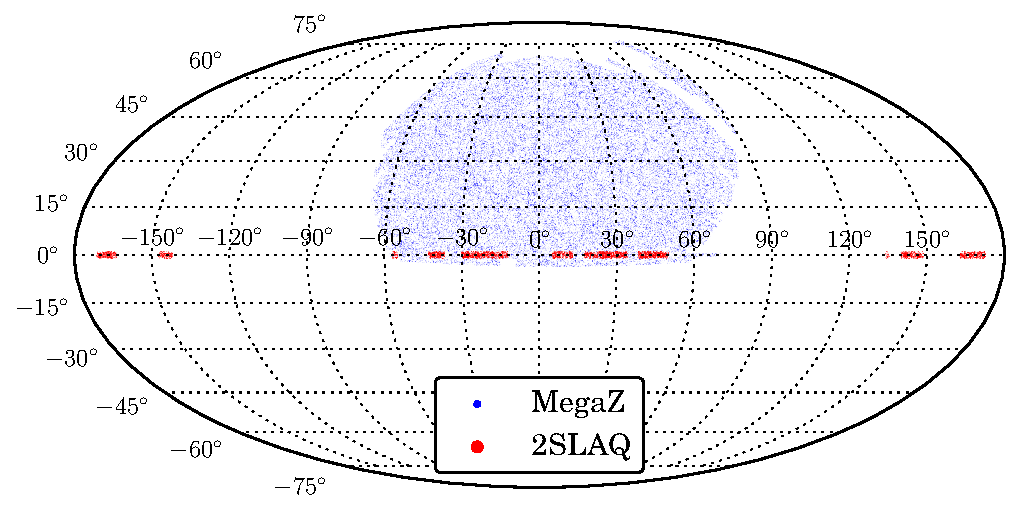
\includegraphics[type=pdf,ext=.pdf,read=.pdf, width=130mm]{./plots/scatter_map}
\caption{Mega-Z and 2SLAQ maps in Mollweide projection plotted in blue and red respectively. For the sake of clarity only a hundred thousand galaxies randomly selected from Mega-Z and five thousand from 2SLAQ have been plotted. The Mega-Z sample covers a total of 7750~deg$^2$, while 2SLAQ covers 180~deg$^2$. The 2SLAQ area is divided into several fields inside a 2$^\circ$-wide strip that extends along the celestial equator.} 
\label{scatter_map}
\end{figure*}

In order to calibrate the photometric redshifts of the Mega-Z galaxies, a representative galaxy sample with known redshifts is needed.  Fortunately, such a sample exists: the 2dF-SDSS LRG and Quasar\footnote{The whole 2SLAQ data can be downloaded from \url{http://www.2slaq.info/query/2slaq_LRG_webcat_hdr.txt.}} (2SLAQ) catalog \citep{Cannon2006} was obtained using the same selection criteria as the Mega-Z catalog and includes $\sim$13100 LRGs with spectroscopic redshifts. Its sky coverage of only 180~deg$^2$ can be seen in Fig.~\ref{scatter_map} in red. The galaxies are located on a strip of 2~deg along the celestial equator, the area subtended by the 2dF spectrograph. Only non-repeated objects ($ind=1$) with high spectroscopic redshift confidence level ($hqs\ge3$) are used in this analysis. 

The selection criteria in both catalogs consist of a magnitude cut and several color cuts. All magnitudes have been corrected for galactic extinction;  we use model magnitudes for the color cuts and to compute the photometric redshifts (section~\ref{sec:photoz}). The magnitude cut 
\begin{equation}
17.5<i_{deV}<19.8
\label{mag_cut}
\end{equation}
is motivated by the limiting magnitude of the 2dF spectrograph and to ensure completeness of the 2SLAQ catalog. While the Mega-Z catalog is complete up to magnitude $i_{deV}=20$, the 2SLAQ completeness drops off sharply beyond $i_{deV}=19.8$, so the cut forces us to cut the Mega-Z sample at this limit. It eliminates $\sim$32\% of the Mega-Z galaxies leaving a total of $\sim$950000. The $i_{deV}$ magnitude distribution for both samples is plotted on the bottom-right of Fig.~\ref{Nm_megaz}. The purple lines represent the cut in~(\ref{mag_cut}).

\begin{figure*}
\centering
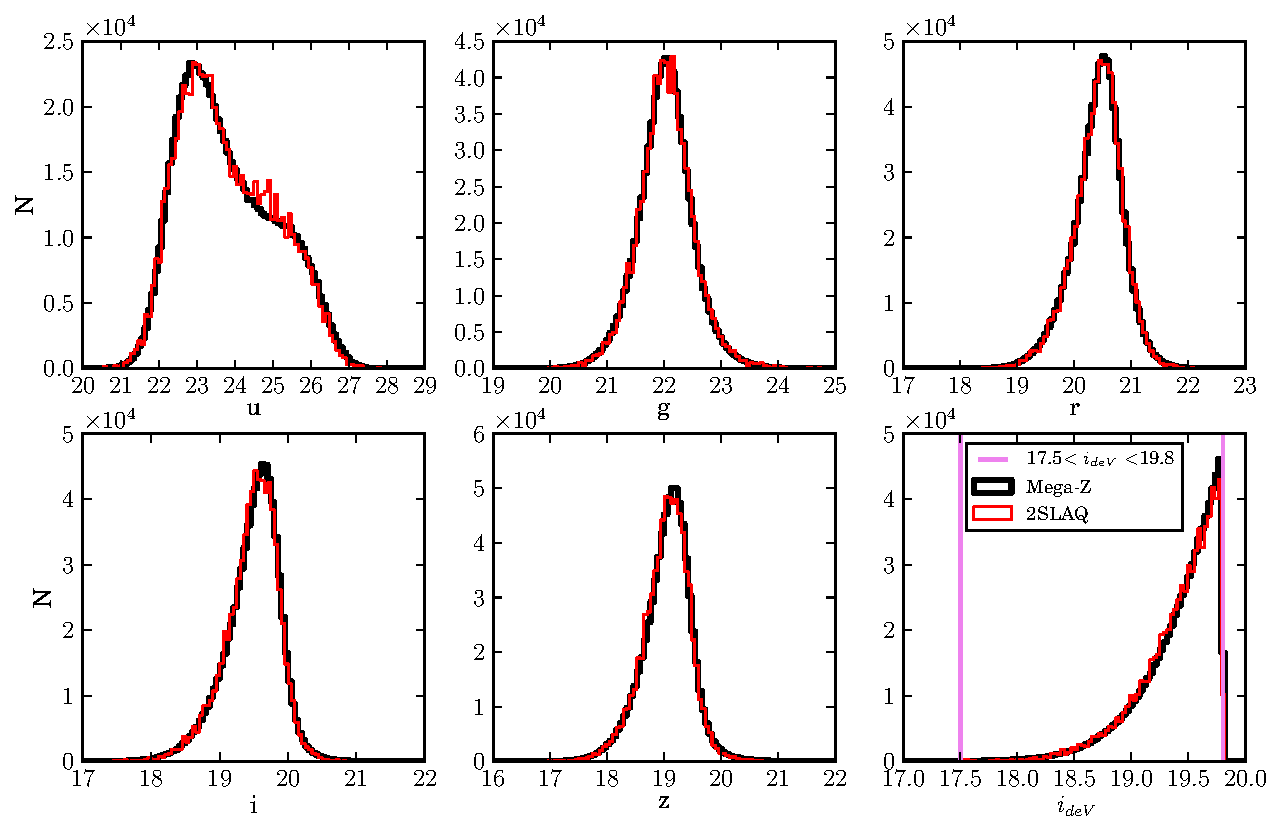
\includegraphics[type=pdf,ext=.pdf,read=.pdf, width=150mm]{./plots/Nm_megaz}
\caption{From top-left to bottom-right, the model magnitude distributions in the $ugriz$ bands for 2SLAQ in red and Mega-Z in black, normalized to each other. The last plot corresponds to the $i$ band de Vaucouleurs magnitude. All magnitudes are corrected for galactic extinction. The purple lines in the last plot show the magnitude cut 
in~(\ref{mag_cut}), which is the nominal limiting magnitude for the 2SLAQ sample. The agreement is excellent, except in the $u$ band, where the low signal-to-noise produces a small disagreement around magnitude $\sim$25.}
\label{Nm_megaz}
\end{figure*}

The color cuts applied are: 
\begin{eqnarray}
0.5<g-r&<&3 \label{gr_isol_lrg}\\
r-i&<&2 \label{ri_isol_lrg}\\
c_\parallel \equiv 0.7(g-r)+1.2(r-i-0.18)&>&1.6 \label{later_type}\\
d_\perp \equiv (r-i)-(g-r)/8.0&>&0.55 \label{zp_cut} \, .
\end{eqnarray}
They are used to isolate the LRGs from the rest of galaxies. In particular, (\ref{later_type}) separates later-type galaxies from LRGs, and (\ref{zp_cut}) acts as an implicit photo-z cut of $z\gtrsim0.45$, as we will see in the next section.
In~\citet{Collister2007} the $d_\perp$ cut is set to 0.5 for the Mega-Z catalog, but, once again, the 2SLAQ completeness within $0.5<d_\perp<0.55$ is very poor: once all other cuts are applied, they represent 3.6\% of the galaxies, instead of 27\% in Mega-Z. Therefore, we choose $d_\perp > 0.55$.

These magnitude and color cuts leave a total of 749152 objects in the Mega-Z catalog and 11810 in the 2SLAQ catalog. In Figs.~\ref{Nm_megaz} and \ref{colors_megaz}, we plot the model magnitude distributions and the color-color scatters, respectively, for all the $ugriz$ bands, after applying all cuts. 2SLAQ is shown in red and Mega-Z in black. Solid and dashed lines represent the cuts. The 2SLAQ magnitude distributions have been normalized up to the total amount of galaxies in Mega-Z. The agreement between both catalogs is excellent, so that we can conclude that 2SLAQ is a representative spectroscopic sample of Mega-Z.
\begin{figure*}
\centering
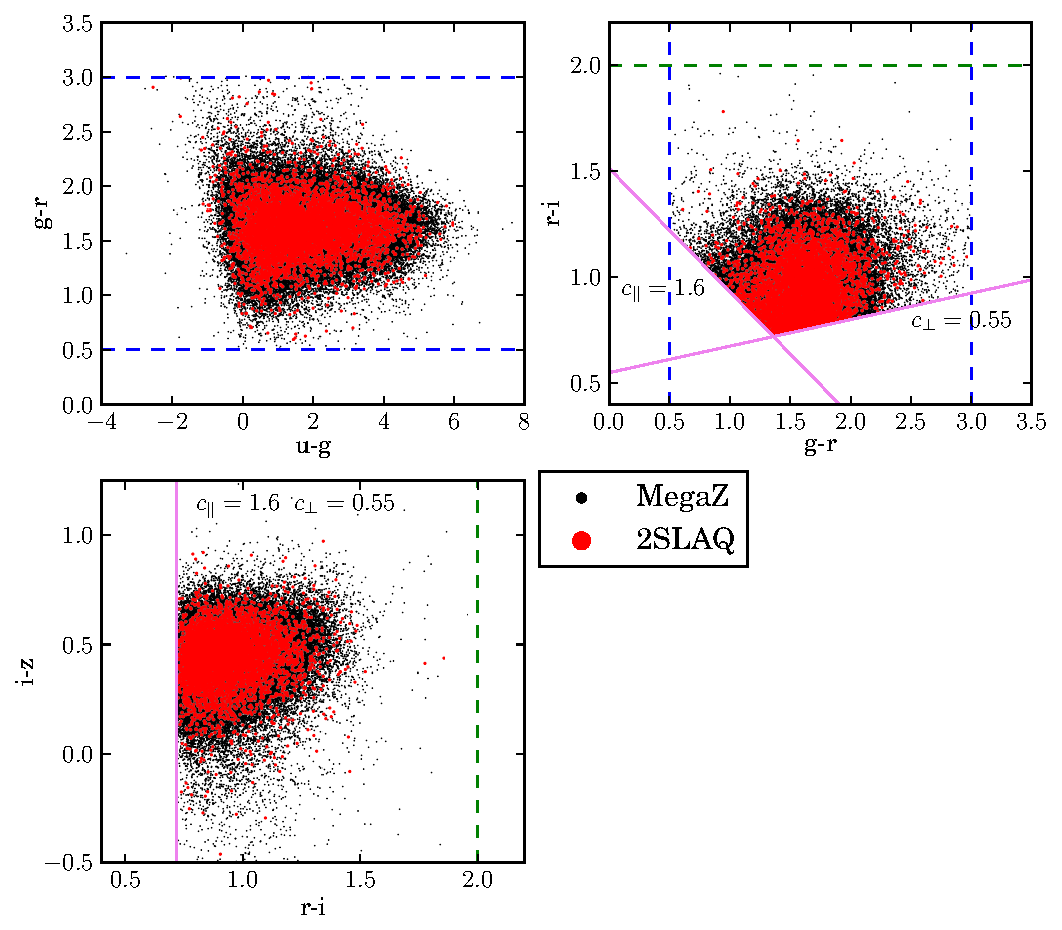
\includegraphics[type=pdf,ext=.pdf,read=.pdf, width=130mm]{./plots/colors_megaz}
\caption{Color-color diagrams for both the Mega-Z catalog in black and the 2SLAQ catalog in red. For the sake of clarity, we have only plot a hundred-thousand galaxies for Mega-Z and five thousand for 2SLAQ. We can see that 2SLAQ covers the same color area as Mega-Z, so that we can conclude that it is a good representative spectroscopic sample. The blue and green dashed lines show the color cuts in (\ref{gr_isol_lrg}) and (\ref{ri_isol_lrg}) respectively, while the purple solid lines show the cuts in (\ref{later_type}) and (\ref{zp_cut}), used to select LRGs and high-z galaxies, respectively. The two last cuts shown in the top-right plot translate into an implicit cut of $r-i>0.72$ in the bottom plot.}
\label{colors_megaz}
\end{figure*}

Additionally, some extra cuts have been applied in the Mega-Z catalog to reduce the star contamination:
\begin{eqnarray}
i_{psf}-i_{model}&>&0.2\times(21.0-i_{deV})\\
i\text{-band de Vaucouleurs radius}&>&0.2\\
\delta_{sg} &>& 0.2
\end{eqnarray}
As explained in~\citet{Collister2007}, the first two cuts separate galaxies from stars leaving a residual $\sim$5\% contamination of M-type stars, which cannot be trivially separated either using $gri$ colors or through cuts on the subtended angular diameter. Because of this, the last cut is applied. First, the photo-z neural network ANNz~\citep{Collister2004} is trained on the 2SLAQ catalog that contains reliable information about whether objects are stars or galaxies. The trained network is then run on the whole Mega-Z catalog to compute the probability $\delta_{sg}$ that objects be galaxies. Removing all objects with probability below 0.2 reduces the stellar contamination from 5\% to 2\%~\citep{Collister2007}. In 2SLAQ, we can remove stars by simply getting rid of all those objects with redshift less than 0.01. 
